% ============================================================
% SECCIÓN 3.4 - DESARROLLO Y ARQUITECTURA DE KUITI
% ============================================================
% Nota: Los diagramas están en formato PlantUML en la carpeta /diagramas/
% Generar las imágenes con: java -jar plantuml.jar diagramas/*.puml -o ../imgs/diagramas/

% 3.4 Arquitectura y Desarrollo de Kuiti
% ===========================================================
\section[Arquitectura de Kuiti]{Desarrollo y Arquitectura de la Aplicación Kuiti}
\label{sec:arquitectura_kuiti}

Kuiti es un asistente universitario inteligente desarrollado como aplicación nativa Android, diseñado para proporcionar información instantánea sobre trámites, reglamentos y servicios de la Universidad Tecnológica de la Mixteca (UTM). El nombre \textit{Kuiti} proviene del mixteco y significa ``veloz'' o ``rápido'', reflejando la filosofía del proyecto de brindar respuestas ágiles a las consultas estudiantiles.

La arquitectura de la aplicación sigue el patrón \textbf{MVVM (Model-View-ViewModel)} combinado con principios de \textbf{Clean Architecture}, garantizando separación de responsabilidades, testabilidad y mantenibilidad del código.

\vspace{1em}
% -----------------------------------------------------------
\subsection{Arquitectura General del Sistema}
\label{subsec:arquitectura_general}

El sistema Kuiti está compuesto por tres capas principales que interactúan entre sí de manera desacoplada: la capa de presentación (UI), la capa de dominio (ViewModel) y la capa de datos (Repository/API).

\subsubsection{Diagrama de Arquitectura MVVM}
\label{subsubsec:diagrama_mvvm}

La arquitectura implementa el flujo unidireccional de datos, donde la UI observa cambios en el estado mediante \texttt{StateFlow} de Kotlin Coroutines. El sistema se divide en tres capas bien definidas.

% Diagrama 3.4.1: Capas UI y Domain
\begin{figure}[h!]
\centering
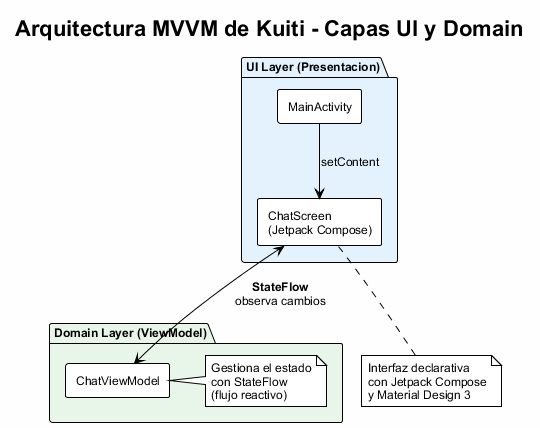
\includegraphics[width=0.80\textwidth]{imgs/diagramas/arquitectura_mvvm_parte1.png}
\caption{Figura 3.4.1: Arquitectura MVVM de Kuiti - Capas de Presentacion y Dominio}
\label{fig:arquitectura_mvvm_parte1}
\end{figure}

% Diagrama 3.4.2: Capa de Datos
\begin{figure}[h!]
\centering
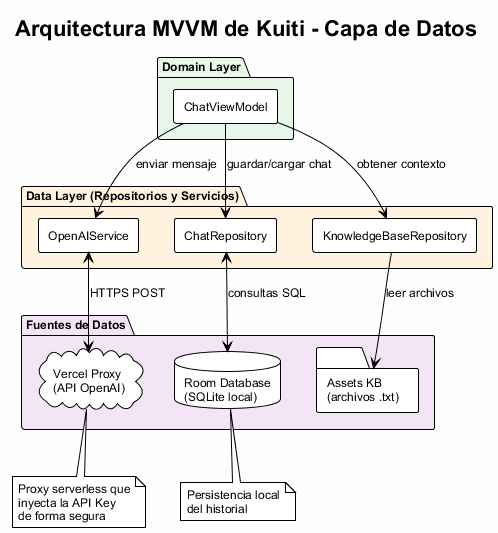
\includegraphics[width=0.85\textwidth]{imgs/diagramas/arquitectura_mvvm_parte2.png}
\caption{Figura 3.4.2: Arquitectura MVVM de Kuiti - Capa de Datos y Fuentes}
\label{fig:arquitectura_mvvm_parte2}
\end{figure}

\vspace{0.5em}

El flujo de datos sigue el siguiente proceso:
\begin{enumerate}
    \item El usuario interactúa con \texttt{ChatScreen} (interfaz Jetpack Compose).
    \item Las acciones del usuario invocan métodos en \texttt{ChatViewModel}.
    \item El ViewModel coordina las operaciones entre repositorios y servicios.
    \item Los cambios de estado se propagan mediante \texttt{StateFlow} hacia la UI.
\end{enumerate}

\vspace{1em}
% -----------------------------------------------------------
\subsection{Estructura de Paquetes y Componentes}
\label{subsec:estructura_paquetes}

La organizacion del codigo sigue una estructura modular que facilita la navegacion y el mantenimiento. El proyecto se divide en dos capas principales: \texttt{data} para la logica de datos y \texttt{ui} para la presentacion.

% Diagrama 3.4.3: Estructura de datos - Servicios y Persistencia
\begin{figure}[h!]
\centering
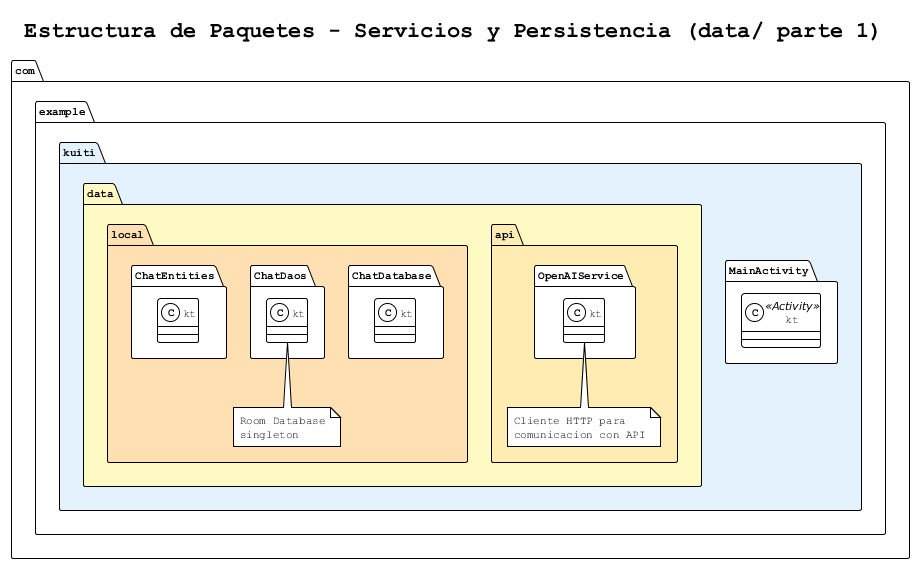
\includegraphics[width=0.75\textwidth]{imgs/diagramas/estructura_paquetes_parte1.png}
\caption{Figura 3.4.3: Estructura de paquetes - Servicios y Persistencia (data/ parte 1)}
\label{fig:estructura_paquetes_parte1}
\end{figure}

% Diagrama 3.4.4: Estructura UI y Temas
\begin{figure}[h!]
\centering
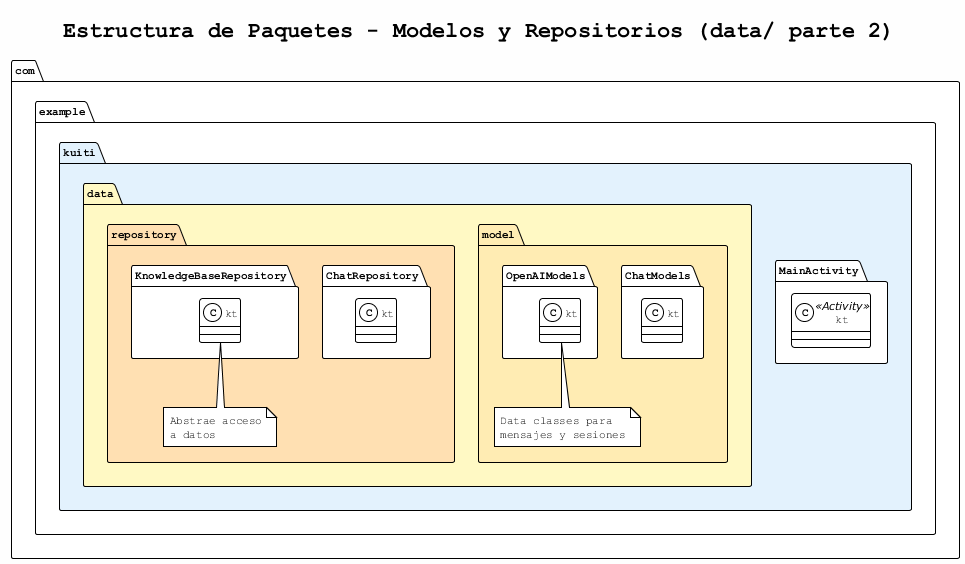
\includegraphics[width=0.75\textwidth]{imgs/diagramas/estructura_paquetes_parte3.png}
\caption{Figura 3.4.4: Estructura de paquetes - Modelos y Repositorios (data/ parte 2)}
\label{fig:estructura_paquetes_parte3}
\end{figure}

% Diagrama 3.4.5: Capa de Presentacion
\begin{figure}[h!]
\centering
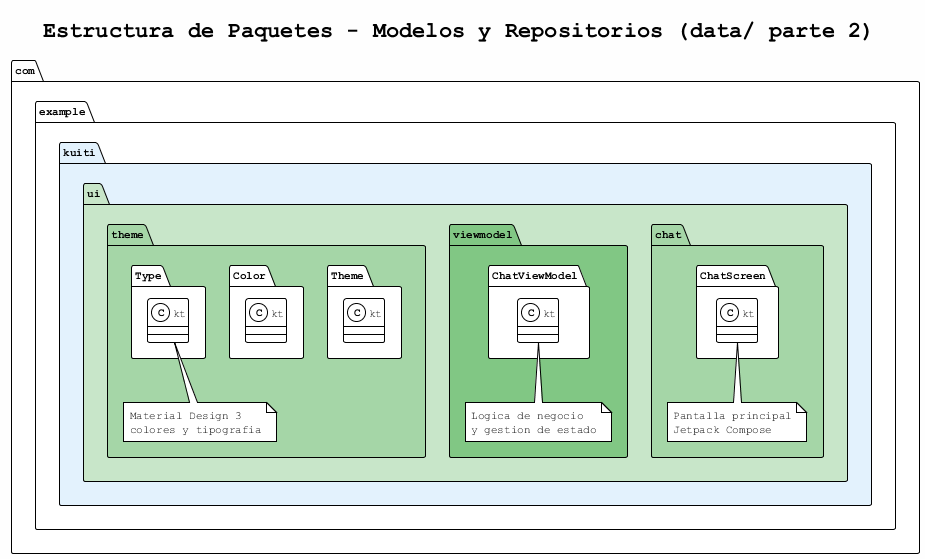
\includegraphics[width=0.75\textwidth]{imgs/diagramas/estructura_paquetes_parte2.png}
\caption{Figura 3.4.5: Estructura de paquetes - Capa de Presentacion (ui/)}
\label{fig:estructura_paquetes_parte2}
\end{figure}

\begin{itemize}
    \item \textbf{data/api:} Contiene el servicio para comunicacion con la API de OpenAI.
    \item \textbf{data/local:} Implementacion de Room Database para persistencia local.
    \item \textbf{data/model:} Clases de datos (Data Classes) para el modelo de dominio.
    \item \textbf{data/repository:} Repositorios que abstraen el acceso a datos.
    \item \textbf{ui/chat:} Componentes de interfaz con Jetpack Compose.
    \item \textbf{ui/viewmodel:} ViewModels para gestion del estado.
    \item \textbf{ui/theme:} Configuracion de Material Design 3.
\end{itemize}

\vspace{1em}
% -----------------------------------------------------------
\subsection{Capa de Datos y Persistencia}
\label{subsec:capa_datos}

La capa de datos implementa el patrón Repository para abstraer las fuentes de datos y proporcionar una interfaz limpia al ViewModel.

\subsubsection{Base de Datos Local con Room}
\label{subsubsec:room_database}

La persistencia del historial de conversaciones se implementa mediante Room, el ORM oficial de Android.

\begin{lstlisting}[style=angelcode,language=Kotlin,caption={Definición de entidades Room para persistencia}]
@Entity(tableName = "chat_sessions")
data class ChatSessionEntity(
    @PrimaryKey val id: String,
    val title: String,
    val createdAt: Long,
    val updatedAt: Long
)

@Entity(
    tableName = "messages",
    foreignKeys = [ForeignKey(
        entity = ChatSessionEntity::class,
        parentColumns = ["id"],
        childColumns = ["sessionId"],
        onDelete = ForeignKey.CASCADE
    )],
    indices = [Index(value = ["sessionId"])]
)
data class MessageEntity(
    @PrimaryKey val id: String,
    val sessionId: String,
    val content: String,
    val isFromUser: Boolean,
    val timestamp: Long,
    val isError: Boolean = false
)
\end{lstlisting}

% Diagrama 3.4.6: Diagrama E-R
\begin{figure}[h!]
\centering
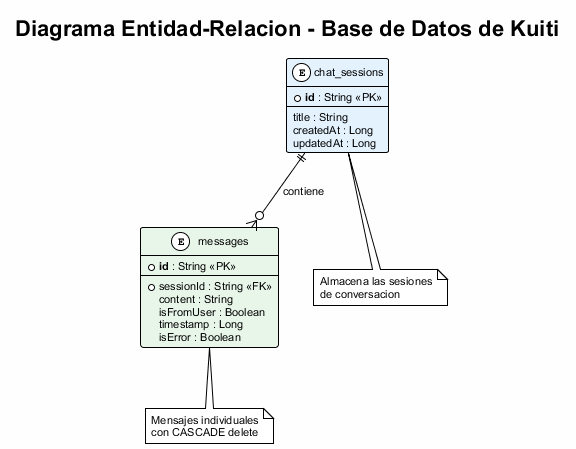
\includegraphics[width=0.70\textwidth]{imgs/diagramas/diagrama_er.png}
\caption{Figura 3.4.6: Diagrama Entidad-Relacion - Base de Datos de Kuiti}
\label{fig:diagrama_er}
\end{figure}

\subsubsection{Sistema de Base de Conocimiento}
\label{subsubsec:knowledge_base}

El repositorio de conocimiento carga documentos de texto desde la carpeta \texttt{assets/kb/} y genera el contexto del sistema para el modelo de lenguaje.

\begin{lstlisting}[style=angelcode,language=Kotlin,caption={Generación del contexto del sistema}]
fun generateSystemContext(): String {
    val documents = loadAllDocuments()
    val contextBuilder = StringBuilder()
    contextBuilder.append(getDefaultSystemPrompt())
    contextBuilder.append("\n\n=== BASE DE CONOCIMIENTO ===\n\n")
    
    for (doc in documents) {
        contextBuilder.append("--- ${doc.type.name}: ${doc.name} ---\n")
        contextBuilder.append(doc.content)
        contextBuilder.append("\n\n")
    }
    return contextBuilder.toString()
}
\end{lstlisting}

\begin{table}[h!]
\centering
\caption{Archivos de la Base de Conocimiento de Kuiti}
\label{tab:knowledge_base_files}
\renewcommand{\arraystretch}{1.2}
\begin{tabular}{@{}p{4.5cm}p{4cm}p{5.5cm}@{}}
\toprule
\textbf{Archivo} & \textbf{Tipo} & \textbf{Contenido} \\
\midrule
reglamento\_licenciatura.txt & REGLAMENTO & Reglamento de estudios de licenciatura \\
\midrule
admision.txt & ADMISION & Proceso de admisión e inscripciones \\
\midrule
licenciaturas\_posgrados.txt & LICENCIATURAS & Oferta educativa disponible \\
\midrule
becas.txt & BECAS & Información sobre becas disponibles \\
\midrule
servicios\_escolares.txt & TRAMITES & Servicios y trámites escolares \\
\midrule
calendario\_escolar.txt & CALENDARIO & Fechas importantes del ciclo \\
\midrule
general\_utm.txt & GENERAL & Información general de la UTM \\
\bottomrule
\end{tabular}
\end{table}

\vspace{1em}
% -----------------------------------------------------------
\subsection{Integración con API de OpenAI}
\label{subsec:integracion_openai}

La comunicación con el modelo de lenguaje se realiza a través de un proxy serverless desplegado en Vercel, lo que permite mantener segura la API key de OpenAI.

\subsubsection{Arquitectura del Flujo de Comunicación}
\label{subsubsec:flujo_api}

% Diagrama 3.4.7: Diagrama de secuencia
\begin{figure}[h!]
\centering
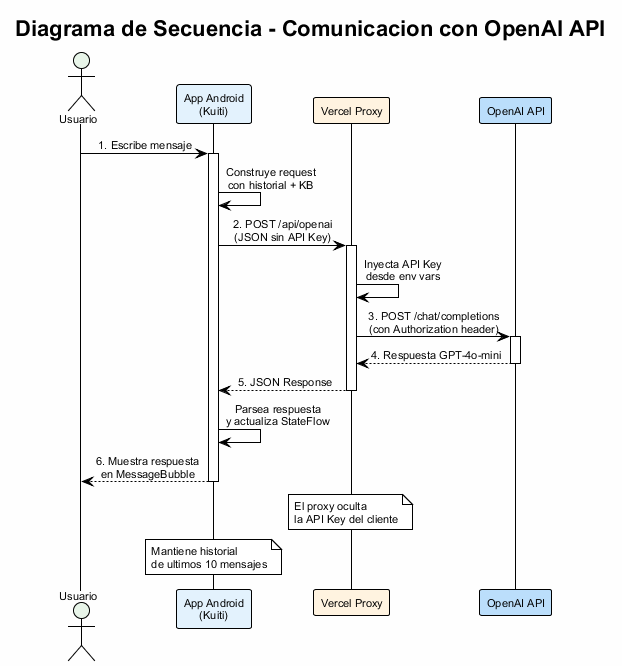
\includegraphics[width=0.90\textwidth]{imgs/diagramas/secuencia_api.png}
\caption{Figura 3.4.7: Diagrama de Secuencia - Comunicacion con OpenAI API}
\label{fig:secuencia_api}
\end{figure}

\subsubsection{Servicio de OpenAI}
\label{subsubsec:openai_service}

\begin{lstlisting}[style=angelcode,language=Kotlin,caption={Implementación del servicio OpenAI}]
class OpenAIService {
    private val client = OkHttpClient.Builder()
        .connectTimeout(30, TimeUnit.SECONDS)
        .readTimeout(60, TimeUnit.SECONDS)
        .build()
    
    private val baseUrl = "https://api-eta-two-34.vercel.app/api/openai"
    
    suspend fun sendMessage(
        systemPrompt: String,
        conversationHistory: List<OpenAIMessage>,
        userMessage: String
    ): Result<String> = withContext(Dispatchers.IO) {
        val messages = mutableListOf<OpenAIMessage>()
        messages.add(OpenAIMessage(role = "system", content = systemPrompt))
        messages.addAll(conversationHistory.takeLast(10))
        messages.add(OpenAIMessage(role = "user", content = userMessage))
        
        val request = OpenAIRequest(
            messages = messages,
            max_tokens = 1024,
            temperature = 0.7
        )
        // ... envío y procesamiento de respuesta
    }
}
\end{lstlisting}

\vspace{1em}
% -----------------------------------------------------------
\subsection{Capa de Presentación con Jetpack Compose}
\label{subsec:capa_presentacion}

La interfaz de usuario está construida completamente con Jetpack Compose, el toolkit moderno de UI declarativa de Android, implementando Material Design 3.

\subsubsection{Componentes Principales de UI}
\label{subsubsec:componentes_ui}

La interfaz se construye mediante composables anidados que siguen el patron de composicion de Jetpack Compose.

% Diagrama 3.4.8: Componentes UI parte 1
\begin{figure}[h!]
\centering
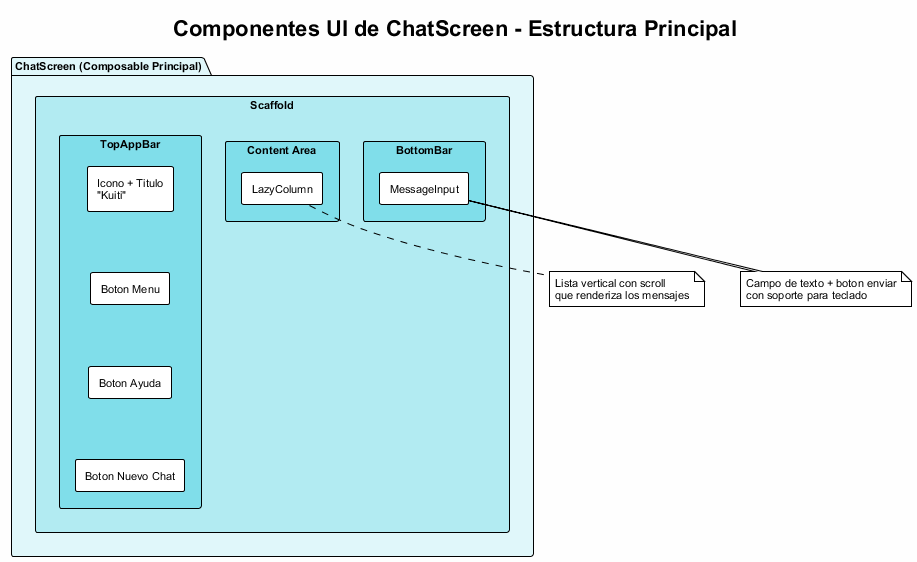
\includegraphics[width=0.80\textwidth]{imgs/diagramas/componentes_ui_parte1.png}
\caption{Figura 3.4.8: Componentes UI de ChatScreen - Estructura Principal}
\label{fig:componentes_ui_parte1}
\end{figure}

% Diagrama 3.4.9: Componentes UI parte 2
\begin{figure}[h!]
\centering
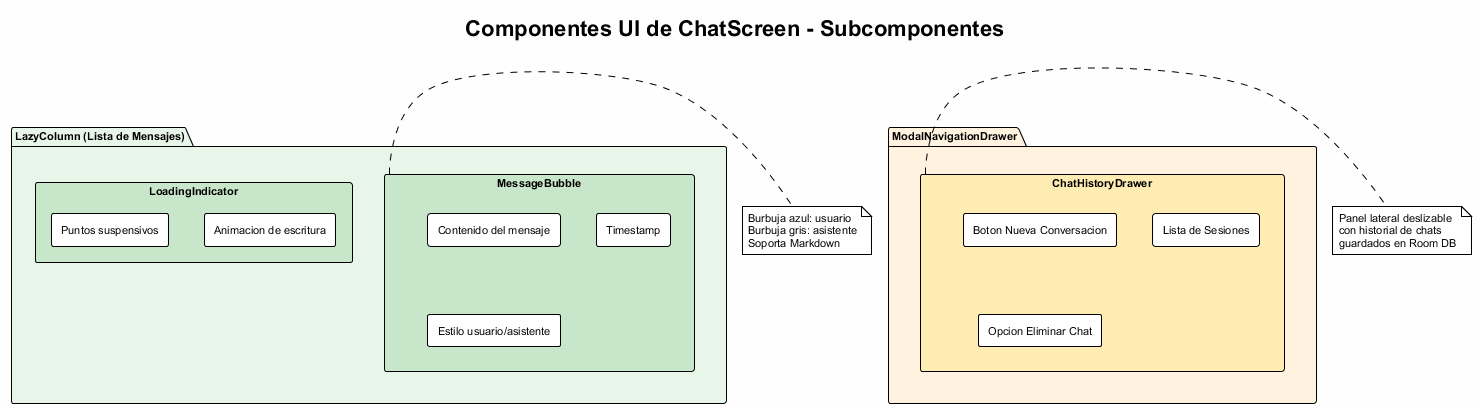
\includegraphics[width=0.80\textwidth]{imgs/diagramas/componentes_ui_parte2.png}
\caption{Figura 3.4.9: Componentes UI de ChatScreen - Subcomponentes}
\label{fig:componentes_ui_parte2}
\end{figure}

\begin{lstlisting}[style=angelcode,language=Kotlin,caption={Estructura principal de ChatScreen}]
@Composable
fun ChatScreen(
    chatState: ChatState,
    historyState: ChatHistoryState,
    onSendMessage: (String) -> Unit,
    onClearChat: () -> Unit,
    onNewChat: () -> Unit,
    onLoadChat: (String) -> Unit,
    onDeleteChat: (String) -> Unit,
    modifier: Modifier = Modifier
) {
    ModalNavigationDrawer(
        drawerState = drawerState,
        drawerContent = { ChatHistoryDrawer(...) }
    ) {
        Scaffold(
            topBar = { TopAppBar(...) },
            bottomBar = { MessageInput(...) }
        ) { paddingValues ->
            LazyColumn(...) {
                items(chatState.messages) { message ->
                    MessageBubble(message = message)
                }
            }
        }
    }
}
\end{lstlisting}

\vspace{1em}
% -----------------------------------------------------------
\subsection{Gestión del Estado con ViewModel}
\label{subsec:gestion_estado}

El \texttt{ChatViewModel} centraliza toda la lógica de negocio y gestiona el estado de la aplicación mediante \texttt{StateFlow}.

% Diagrama 3.4.10: Diagrama de estados
\begin{figure}[h!]
\centering
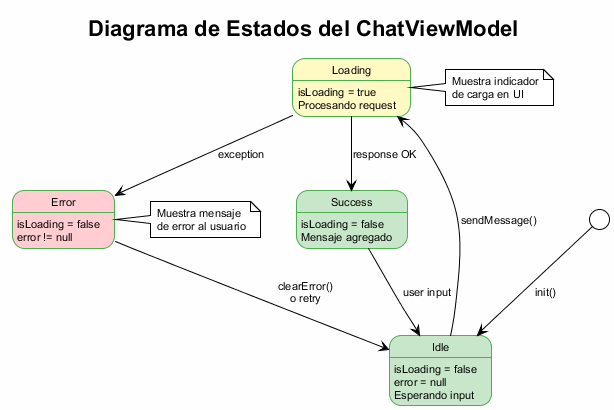
\includegraphics[width=0.70\textwidth]{imgs/diagramas/estados_viewmodel.png}
\caption{Figura 3.4.10: Diagrama de Estados del ChatViewModel}
\label{fig:estados_viewmodel}
\end{figure}

\begin{lstlisting}[style=angelcode,language=Kotlin,caption={Definición del estado del chat}]
data class ChatState(
    val currentSessionId: String? = null,
    val messages: List<Message> = emptyList(),
    val isLoading: Boolean = false,
    val error: String? = null
)

data class ChatHistoryState(
    val sessions: List<ChatSession> = emptyList(),
    val isDrawerOpen: Boolean = false
)
\end{lstlisting}

\vspace{1em}
% -----------------------------------------------------------
\subsection{Stack Tecnológico y Dependencias}
\label{subsec:stack_tecnologico}

La aplicación utiliza las tecnologías más modernas del ecosistema Android.

\begin{table}[h!]
\centering
\caption{Stack tecnológico de Kuiti}
\label{tab:stack_tecnologico}
\renewcommand{\arraystretch}{1.3}
\begin{tabular}{@{}p{3.5cm}p{3.5cm}p{7cm}@{}}
\toprule
\textbf{Categoría} & \textbf{Tecnología} & \textbf{Propósito} \\
\midrule
Lenguaje & Kotlin 1.9+ & Lenguaje principal de desarrollo \\
\midrule
UI Framework & Jetpack Compose & Interfaz declarativa y reactiva \\
\midrule
Diseño & Material Design 3 & Sistema de diseño moderno \\
\midrule
Arquitectura & MVVM + Clean & Separación de responsabilidades \\
\midrule
Persistencia & Room Database & Base de datos local SQLite \\
\midrule
Networking & OkHttp + Gson & Cliente HTTP y serialización JSON \\
\midrule
Concurrencia & Kotlin Coroutines & Operaciones asíncronas \\
\midrule
Estado & StateFlow & Gestión reactiva del estado \\
\midrule
Backend & Vercel Serverless & Proxy API para seguridad \\
\midrule
IA & OpenAI GPT-4o-mini & Modelo de lenguaje para respuestas \\
\bottomrule
\end{tabular}
\end{table}

\vspace{1em}
% -----------------------------------------------------------
\subsection{Consideraciones de Seguridad y Despliegue}
\label{subsec:seguridad_despliegue}

\begin{itemize}
    \item \textbf{Protección de API Key:} La clave de OpenAI nunca se incluye en el código fuente de la aplicación. Se utiliza un proxy serverless en Vercel que inyecta la clave de forma segura.
    \item \textbf{Datos locales:} El historial de conversaciones se almacena únicamente en el dispositivo del usuario mediante Room Database, sin transmisión a servidores externos.
    \item \textbf{Comunicación segura:} Todas las comunicaciones con la API utilizan HTTPS.
    \item \textbf{Compatibilidad:} SDK mínimo 24 (Android 7.0), target SDK 35 (Android 15).
\end{itemize}

\vspace{1em}
% -----------------------------------------------------------
\subsection{Extensibilidad y Trabajo Futuro}
\label{subsec:extensibilidad}

\begin{itemize}
    \item \textbf{Objetivo principal:} Proporcionar un asistente virtual accesible que reduzca la carga de consultas en Servicios Escolares de la UTM.
    \item \textbf{Aplicaciones potenciales:} Integración con sistemas institucionales, notificaciones push para fechas importantes, soporte multiidioma incluyendo lenguas originarias.
    \item \textbf{Limitaciones conocidas:} Dependencia de conexión a internet para consultas IA, base de conocimiento estática que requiere actualización manual.
    \item \textbf{Extensiones posibles:} Implementación de RAG (Retrieval-Augmented Generation) para consultas más precisas, integración con calendario institucional en tiempo real, soporte offline con modelo local.
\end{itemize}

\vspace{0.5em}

\noindent En síntesis, Kuiti representa una implementación moderna de un asistente virtual universitario, combinando tecnologías de vanguardia como Jetpack Compose, Kotlin Coroutines y modelos de lenguaje GPT para ofrecer una experiencia de usuario fluida y respuestas contextualizadas sobre la vida académica en la UTM. La arquitectura MVVM y el uso de patrones de diseño establecidos garantizan un código mantenible y extensible para futuras mejoras.

% --- Fin de sección 3.4 ---
